\chapter{Background}\label{sec:background}

    \begin{blockquote}
        \paragraph{Intent:} General background information needed to follow the terms and methods used in this thesis. 
                
        Structure:
        \begin{description}
            \item[1. Parameter tuning] Parameter tuning of a black-box
                \begin{enumerate}
                    \item $f(Parameter) = Objective$ 
                    \item Goal is optimize $f$
                    \item Problem: Optimization of multiple objectives
                \end{enumerate}
            \item[2. Multi-objective optimization] General definition. Pareto front and None-dominated solution
                \begin{enumerate}
                    \item What is a multi-objective solution?
                    \item How to compare solutions? $\rightarrow$ Types of metrics
                    \item How to solve? $\rightarrow$ Scalarizing, MOEA, Random
                    \item Problem: Reduce evaluations $\rightarrow$ Surrogate optimization, MBMO
                \end{enumerate}
            \item[3. Surrogate optimization] Approach for reducing evaluation count
                \begin{enumerate}
                    \item Intro. Cons and Pons
                    \item Types of a surrogate model in a MO-problem (Model of scalarization, MO-model, Replicated MO-model, Compositional MO-model). Taxonomy
                    \item Surrogate assistance for MO parameter tuning $\rightarrow$ Reusable/scalable components for optimization $\rightarrow$ Problem: Scalability of a surrogate model.                  
                    \item Surrogate model is domain-specific $\rightarrow$ Analyze multiple surrogates $\rightarrow$ Surrogate portfolio [RQ1 \ref{RQ1}]
                    \item Sampling plan. Build a surrogate model. Quality of prediction depends on the accuracy of a surrogate model  $\rightarrow$ Accuracy depends on a sample size $\rightarrow$ Sample size depends on surface type $\rightarrow$ Problem: Sample size is static. [RQ2 \ref{RQ2}]
                    \item Surrogates and MOEA are hard scalable 
                \end{enumerate}
            \item[4. Scope of work] Starting point of thesis
                \begin{enumerate}
                    \item Problem: Expensive black-box with multiple objectives
                    \item Constraint: Evaluation budget
                    \item Goal: Set of MO solutions closed to Pareto-front $\rightarrow$ 1.$Max$ Hypervolume, 2.$Min$ Points-Space, 3.$Max$ \% of None-Dominated points 
                    \item Solution approach: Surrogate model(s) with MOEA
                \end{enumerate}
        \end{description}
    \end{blockquote}

    This chapter presents general background information needed to follow the terms and methods used in this thesis. 

    % --------------------------------------------------------------------------------------------
    % ------------------------------------------------        Parameter tuning
    % --------------------------------------------------------------------------------------------
    \section{Parameter tuning}
        We consider fitness function $f$ as a black-box with parameter and objective space. Parameter space has structure and could consist of continuous and categorical dimensions. Sometimes, some combinations of parameter settings are forbidden. Each point from parameter space leads to some point in objective space. This mapping called fitness landscape, and the task for optimization algorithm is to find optimal points in this surface. Regardless of the type of landscape, search often yields qualitatively different behaviour.
        The single criterion in parameter tuning may not be sufficient to characterize the behaviour of the configuration space correctly; Therefore, multiple criteria have to be considered. This objectives also could be described as usual aims as max accuracy, min runtime, min latency, max performance and min error rate and energy. Each objective should gain the best possible value and profit in the system's tradeoff. By default, we consider minimization for all objectives. 

        We consider the following property of parameter tuning:
        \begin{itemize}
            \item Evaluation may be very expensive
            \item Black-box function and sampling budget is unknown
            \item Multi-objectivity
        \end{itemize}

        Ideally, require a method that can explore the search space with limiting evaluations budget. 
    

    % --------------------------------------------------------------------------------------------
    % ------------------------------------------------        Multi-objective       -------------
    % --------------------------------------------------------------------------------------------
    \section{Multi-objective optimization}
        Common parameter tuning problems require the simultaneous optimization of multiple, usually contradictive objectives; Multi-objective optimization deals with such conflicting objectives. It provides a mathematical algorithm to arrive at an optimal design state which accommodates the various criteria demanded by the application. The process of optimizing go orderly and simultaneously. The solution to multi-objective problems is a group of points that placing on a Pareto front. Awareness of the Pareto front allows visualizing appropriate decisions in terms of performance for each objective. For a multi-objective problem, we consider "prediction" as points from parameter space that lead to non-dominated results in objective space. This set of points approximates real Pareto-front. Improving "solution" means that sets of points match better with real Pareto-front.

        % ! definition of non-dominate, pareto front and ...


        Solving techniques for multi-objective problems: 
        \begin{itemize}
            \item Grid search vs Random search
            \item Heuristics and Metaheuristic. (Simulated annealing, Evolutionary algorithm) These methods aim at generating approximately optimal solutions in a single run. It also could operate with sets of solutions, being outcomes of multiple objectives.
            \item Sequential design (Bayesian optimization, Evolutionary algorithm) Bayesian methods differ from random or grid search in that they use past evaluation results to extrapolate and choose the following values to evaluate. Limit expensive evaluations of the objective function by choosing the following input values based on those that have done well in the past.
        \end{itemize}

    % ------------------------------------------------        Metrics       -------------
        \subsection{Metrics for multi-objective solution}
            In single-objective optimization, the quality of a given solution is trivial to quantify. When we consider a solution of a multi-objective problem as a multi-point approximation, comparison of these points is also a multi-objective task.
            The question of metrics for evaluation is essential for the comparison of algorithms or select a point from approximations.

            According to \cite{ZitzlerDT00}, a Pareto front approximation should satisfy the following criteria:
            \begin{itemize}
                \item The distance between the Pareto front and its approximation should be minimized.
                \item A heigh distribution of the non-dominated points is desirable.
                \item The range of the approximated front should be maximized, i.e., for each objective, a wide range of values should be covered by the non-dominated points.
            \end{itemize}

            Metrics for performance indicators partitioned into four groups according to their properties \cite{Audet2018PerformanceII}: cardinality, convergence, distribution and spread. Base on the correct metrics, the general multi-objective algorithm keeps making progress toward the Pareto front in the objective function space.

            The goal of multi-objective optimizing is to obtain an approximation solution set to the reference Pareto front, including the following subgoals:
            \begin{itemize}
                \item All solution set are as close as possible to the Pareto front
                \item All solution set are as diverse as possible in the objective space
                \item The proportion of solutions set to the evaluated set as large as possible. Evaluate as few solutions as feasible.
            \end{itemize}

            Also, distribution and spread indicators are considered in this work. According to \cite{CustodioMVV11}, the spread metrics try to measure the areas of the coverage achieved in a computed Pareto front approximation. This type of metrics is not useful for comparing algorithms or evaluate the convergence of optimization. However, thay could be usefull for a more detailed analysis of the optimization process or for composing Pareto frontier from several solutions.

            For multi-objective optimization, an algorithm should provide a set of solutions that realize the optimal trade-offs between the considered optimization objectives. Therefore, the performance comparison of \gls{moo} algorithms is based on their Pareto sets. In this study, four well-known metrics are used to quantify the performance of the algorithms.
            \begin{itemize}
                \item \textbf{Hypervolume (HV).}\cite{Zitzler2000ComparisonOM} \textit{Convergence and distribution indicator.}
                This metric represents the volume of the objective space that is covered by the individuals of non-dominated solutions set solutions that belong to a Pareto front. Two points delimit the volume: one point is the reference point that is defined as the worst solution inside the objective space, and a second optimal point (pseudo-optimal) that is calculated by the proposed solution method. Establishing the hypervolume indicator is a computationally expensive task. Also, in case of a small dimension and low number of points, there are currently no known algorithms that can return the results fast enough for use in most multiple-objective algorithms.  
                \item \textbf{Non-dominated Ratio (NDR).} \textit{Cardinality.} This metric employs the non-dominated count of a solution set divided by the total size of solution set. Higher values are preferred to lower ones.
                \item \textbf{Spacing \cite{Schott1995FaultTD}.} \textit{Distribution and spread.} Describe the distribution of Pareto points. Fewer space metrics means better coverage of objectives values range. 
                \item \textbf{$\Upsilon$-metric (p-distance)}\cite{Martens13} \textit{Convergence} This metric is the average distance of any set of points to the Pareto front. The lower the $\Upsilon (P)$, the closer the solutions of P are to solutions of the Pareto-front. $\Upsilon(P) = \frac{1}{|P|}\sum_{x\in P}g(x)-g(x^*)$  
            \end{itemize}
 
    % ------------------------------------------------        Solving methods       -------------
        \subsection{Solving methods}
            Generating the Pareto-optimal set often impracticable and can be computationally expensive. Accordingly, many stochastic search strategies have been developed, such as evolutionary algorithms, tabu search, simulated annealing, and ant colony optimization. That algorithms regularly do not ensure to find ideal trade-offs but try to gain a good approximation.
            In this thesis, under the Pareto-optimal front mean an ideal solution to the problem. None-dominated points it is a subset of some feasible points that is none dominated. All points from Pareto-frontier are none-dominated, but not all none-dominated points are Pareto-optimal.

                % ==== dominated
                \begin{figure}
                    \centering 
                    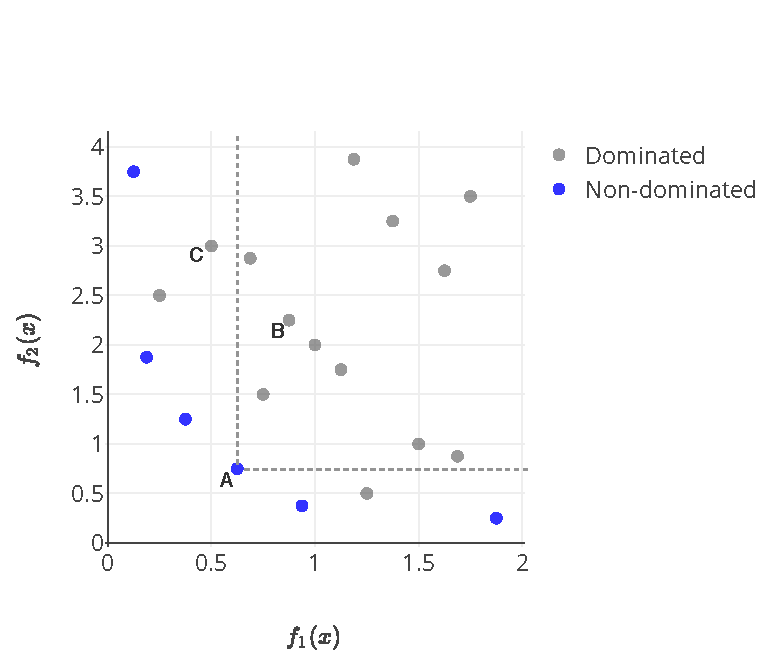
\includegraphics[width=10cm]{content/images/ndom}
                    \caption[Non-dominated points]{Example of non-dominated points. Point A dominated on all points in the internal sector where B is presented. Concerning point A, point B is not dominant because it has better value in $f_1$} 
                    \label{fig:dominated} 
                \end{figure}
        
            % ----------------      Scalarizing       
            \subsubsection{Scalarizing}
                The Scalarizing approach is a popular technique for creating a single-objective \textit{parameterized} problem with the composite criteria from multiple objectives. It folows then single-objective optimization techniques could be applied to this composite function to obtain a single optimal solution. The weighted-sum methods it is a well-known type of scalarizing technic. This approach concatenates the objectives into one criterion by using weighted sum factors. There are difficulties in selecting proper weights, especially when there is no correlation in prior knowledge among objectives.  

                Some scalarizing technics try to improve the exploration of parameter space by assigning more "intelligence" aggregation to the objectives. Such solutions may be fragile. They change dramatically in a modification of algorithm parameters. Moreover, the weighting method can not provide a solution among underparts of the Pareto surface due to the "duality gap" for not convex cases. Also, some of the scalarizing algorithms are very sensitive to the number of objectives. Analysis of the fitness landscape with different scalarizing techniques might be helpful in the optimization for solving expensive MOPs \cite{ChughScal2019}.

                % For example, if we want to reach the point in the middle of two other points in Pareto frontier, we hardly get a peek of the Pareto surface, as long as the well-known simplex method is used. This implies that depending on the structure of the problem. The linearly weighted sum can not necessarily provide a solution as DM desires. \cite{Nakayama05}. Moreover, the weighting method can not provide a solution among underparts of the Pareto surface due to the “duality gap” for not convex cases. 

                % ? Scalable algorithms that convert multi-objective to single-objective problem solve that not accurate enough(Scalarizing). Also, this approach suitable for a limited type of problem. Moreover, there are important lot of parameters that significant influence on algorithm performance.

            % --------------------      MOEA
            \subsubsection{Multi-Objective Evolutionary Algorithms}
            The evolutionary algorithm forms a class of heuristic search methods that simulate the process of natural evolution. An evolutionary algorithm is determined by the two basic principles: selection and variation \cite{TutMOEABrockhoff}. While selection reflects the competition for reproduction and resources among individuals, the other principle, variation, imitates the natural ability to produce new individuals through recombination and mutation. 
            The evolutionary algorithm has several characteristics that are desirable for problems, including multiple conflicting objectives, and large and complicated search spaces. Evolutionary optimizers explore populations of candidate solutions in each generation. Some mutator can make changes to the current population. A select operator then picks the best mutants which are then combined in some way to become generation i+1. However, EA still needs many evaluations of the "black box" system to solve a common multi-objective problem. This expense is further complicated by the fact that many such problems are expensive. This massive evaluations budget makes \gls{ea}s unfeasible for the costly and multi-objective problem. 


    % --------------------------------------------------------------------------------------------
    % ------------------------------------------        Surrogate optimization       -------------
    % --------------------------------------------------------------------------------------------
    \section{Surrogate optimization} 
        The potential for applying surrogate is laid in generalization all search space and fast evaluation. This advantage should outperform disadvantage in time required to build this surrogate model. In classical model-based optimization, single surrogate-model provides a hypothesis on the relation between parameter and objective space. Approximation of the solution becomes faster than real evaluation, so the whole optimization process can be accelerated. On the other hand, the extra time indeed needed to build and update the surrogate models during the optimization process. In the case of pre-selecting the promising individuals, the surrogate model is used to find the probable good candidates or drop the low-quality individuals even before they are exactly evaluated, thus reducing the number of exact evaluations.

        In the literature, the term surrogate or model-based optimization is used where, during the optimization processes, some solutions are not evaluated with the original function, but are approximated using a model of this function. Some of the most commonly used methods are the Response Surface Method \cite{ResponseSurface}, Radial Basis Function \cite{Rasmussen2004}, Neural Network, Kriging \cite{Woodard00}, and Gaussian Process Modeling \cite{RasmussenN10, RasmussenW06}. Surrogates are also used to rank and filter out offspring according to Pareto-related indicators like the hypervolume \cite{EmmerichGN06}, or a weighted sum of the objectives \cite{TaboadaBCW07}. If the model is single-criteria, it could be expanded to multi-objective surrogate by parting each criterion in isolation from the others and duplicating the model for each of them \cite{Knowles06, nardi2019practical}. A surrogate model is either selected randomly or due to its popularity in the associated domain area. Thus there are still some open challenges related to the combination of meta-models, such as the definition of a selection criterion or combination techniques. Besides, there are no guidelines for using heterogeneous compositional models for different objective functions \cite{SoftSurvey}.

        
        % -------------------------------------------------------------------------------------------------
        % ------------------------------------------------        MO in Parameter tuning       -------------
        \subsubsection{Multi-objective parameter tuning}

            The categorization of parameter tuning approaches based on the workflow of sequential model-based optimization \ref{fig:mo_param_tuning}. First, it is the initial sampling plan to generate an early data set to fit surrogate models. As an initial sampling plan or \gls{doe} plan, can use technics as \gls{lhs}, Sobol sampling, or alternative is random sampling.
            
            % ===  Phases and tasks in parameter tuning with surrogates model
            \begin{figure} 
                \centering
                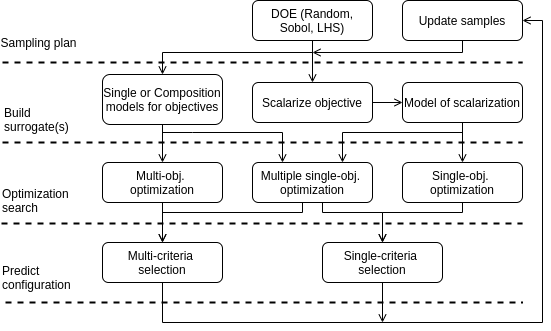
\includegraphics[width=\textwidth]{content/images/tax_mb_tuning}
                \caption[Phases and tasks within a generalized multi-objective parameter tuning]{Phases and tasks within a generalized multi-objective parameter tuning}
                \label{fig:mo_param_tuning}
            \end{figure}

            For extrapolate samples, there are two approaches established. 1) Build surrogates on scalarize objectives and produce a surrogate model as aggregation from objectives. In this case, the multi-objective problem transforms into a single-objective one. 2) Keep original dimensionality of the problem, and apply one or several models to hold and infer on the problem landscape.

            On the next step, the optimization search represents searching for the optimal point(s) with a surrogate model. This step produces candidates for a real evaluation or assumption to the Pareto-optimal points. In the predict configurations phase, sorting and selection are carried out. In the case of multicriteria selection, it is necessary to select the required number of points that are optimal for all quolity criteria. In theory, all points are equal in order to choose them. The advantage of possible prediction several parameters instead of a single one is improving the exploration of the parameter space, and parallelizing of fitness evaluation. The required number of points is allowed to estimate and update the sample set. Optimization iterations continue until the stop condition is satisfied.
    
            The variability and extensibility are essential for configurable parameter tuning, suchlike a software product line. The optimization round is consistent and universal. As shown in Figure \ref{fig:mo_param_tuning}, the potential to reuse components in a workflow is enormous. The same single-objective models can be equally applied to various types of problems in multi-/single-objective optimization. The optimization algorithm weakly depends on the type of surrogate model. Consider improving parameter tuning to multiply criteria on-the-fly by dynamically duplicate surrogate model or even create several variants surrogate hypothesis.

        % --------------------------------------------------------------------------------------------
        % ------------------------------------------------     Domain-specific Surrogate model      
        \subsection{Domain-specific problem}
        Intending to find the best solution with less effort, surrogate models are domain-specific. It could be an interpreter as a \Gls{nfl} in model-based optimization. If we extend this argument, then the same optimization problem in different parameter tuning iteration could be interpreted as another optimization problem. This means that to reduce effort and increase the convergence of an algorithm, we should change the surrogate model depend on how much samples do we have. As one would expect, no approximation method is universal.
        This leads us to use a portfolio with surrogate models. On each optimization, iteration tries several models and selects thous who have the best performance. As a negative consequence, the model fitting introduces an additional overhead into the optimization.


        % --------------------------------------------------------------------------------------------
        % ------------------------------------------------     Build surrogate model     
        \subsection{Initial samples set}
        Initial samples should provide maxim information to build a valuable model. The overall result depends primarily on how well the assumption is valid. It does not matter what the search results are if they have done on the wrong model. Samples maybe not enough, and better select points from initial design than to be guided by an incorrect model. With increasing sample size, in case of proper fitting, a better surrogate model is obtained, and in optimization, is reached better results. On the other hand, the initial sample size may be too big, and it is a waste of resources. 

        Given the type of fitness landscape, the expert can assume how much sample points are required to approximate the objectives. For simple dependencies or more complex surfaces, the difference can be hundreds or thousands of points. Regardless, in the case of the genuinely black-box problem, this information is unknown. Therefore a dynamic sampling plan should be achieved to reduce the number of estimations and improve the convergence of the optimization algorithm.


    % --------------------------------------------------------------------------------------------
    % ------------------------------                    Scope of work       
    \section{Scope of work}
        In this thesis, we focus on improving surrogate models for the multi-objective problem. Surrogate based optimization has proven effective in many aspects of engineering and in applications where data is "expensive", or difficult, to evaluate. While other methods also exist, we select MOEA as main solver because it can apply to a wide range of problems and gives a broad understanding of how Pareto-front might look. Problem type is expensive, multi-objective, derivative-free/black-box system without constraints.

        Design gap in optimization/parameter tuning lay in the quality of the surrogate model:
            \begin{itemize}
                \item Select proper surrogate model
                \item Surrogate composition for multi-dimensional space
                \item Sampling strategy
                \item Surrogate validation
            \end{itemize}

        \paragraph{Goal:}
        \begin{enumerate}
            \item Find diverse solutions with minimal distance to real Pareto frontier.
            \item Reduce the evaluation budget.
            \item Develop modular architecture with extensibility with other frameworks. 
            \item Backwards computationally with sing-objective parameter tuning.
        \end{enumerate}

        Also optimization and composition of multi-objective solvers is a rapidly expanding area of research and a full survey of that work is beyond the scope of this thesis.


    % General classification \cite{MlakarPTF15}:
    % Within surrogate-model-based optimization algorithms, a mechanism is needed to find a balance between the exact and approximate evaluations. In evolutionary algorithms, this mechanism is called evolution control \cite{Jin05} and can be either fixed or adaptive. In fixed evolution control the number of exact function evaluations that will be performed during the optimization is known in advance. Fixed evolution control can be further divided into generation-based control, where in some generations all solutions are approximated and in the others, they are exactly evaluated \cite{DebN07}, and individual based control, where in every generation some (usually the best) solutions are exactly evaluated and others approximated \cite{Grierson1993}. In adaptive evolution control, the number of exactly evaluated solutions is not known in advance but depends on the accuracy of the model for the given problem. Adaptive evolution control can be used in one of two ways: as a part of a memetic search or to pre-select the promising individuals which are then exactly evaluated \cite{PilatN12}.

    % Direct fitness replacement and indirect fitness replacement
    % Kind of extending the search stage of MOEA with surrogate to simulate evaluation of population. It transform the problem of searching a new better population to improving general hypothesis of how and where Pareto set presented.  